\section{Study Settings}

The main goal of this research work is
to understand \ldots
To achieve this general goal, we answer the following
research questions. 


\begin{enumerate}[(RQ1)]
\item research question 1
\item research question 2
\item research question 3
\item \ldots
\end{enumerate}

\subsection{Settings for RQ1}

\subsection{Settings for RQ2}


\begin{figure*}[h!]
  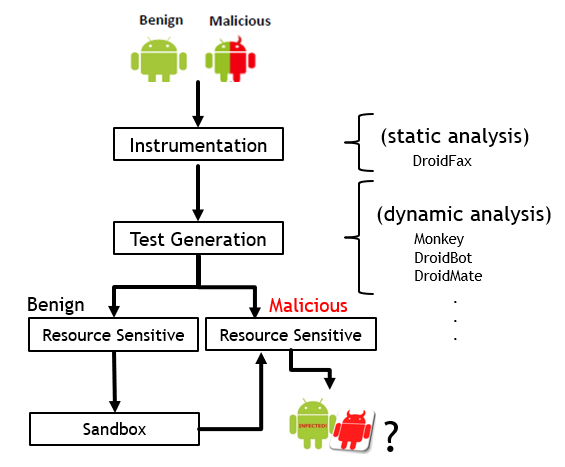
\includegraphics[width=0.5\textwidth]{images/setup.png}
  \label{Experiment setup}
  \caption{Experiment setup}
  \label{fig:setup}
\end{figure*}

To assess the effectiveness of mining sandboxes created by each test case generation tools, we run these tools in benign apps and, based on resources sensitives access in this execution, we build their sandbox. Based on this sandbox, we investigate the capacity of detect malicious behaviors in the corresponding malign app. (Figure  \ref{fig:setup}) show all the experimental setup.

\subsection{Experiment motivation}

As described 
